\documentclass[a4paper,11pt]{article}
\usepackage[margin=1in]{geometry}
\usepackage[T1]{fontenc}
\usepackage{lmodern}
\usepackage{amsmath,amssymb,amsthm,graphicx,booktabs}
\usepackage[hidelinks]{hyperref}
\hypersetup{pdftitle={Certificate Bounds for Backtracking Frank-Wolfe under Function-Dependent Curvature},pdfauthor={Yaroslav P. Lyakhov and Stepan Suvorov}}
\newtheorem{theorem}{Theorem}[section]
\newtheorem{lemma}[theorem]{Lemma}
\newtheorem{proposition}[theorem]{Proposition}
\newtheorem{corollary}[theorem]{Corollary}
\newcommand{\norm}[1]{\left\|#1\right\|}
\newcommand{\inner}[2]{\left\langle#1,#2\right\rangle}
\newcommand{\R}{\mathbb R}
\newcommand{\ceil}[1]{\left\lceil#1\right\rceil}
\DeclareMathOperator{\artanh}{artanh}
\title{Certificate Bounds for Backtracking Frank--Wolfe\\under Function-Dependent Curvature}
\author{Yaroslav P. Lyakhov \and Stepan Suvorov}
\date{15 October 2026}
\begin{document}
\maketitle
\begin{abstract}
We study convex minimization over a compact convex set when the Hessian
norm is bounded by $H_0+H_1(f-f_Q^*)$, relative to the constrained minimum.
For ordinary quadratic backtracking Frank--Wolfe, we prove a bound of
$O(H_0D^2/\varepsilon+(1+H_1D^2)\log(U_0/\varepsilon))$ updates to an
observable certificate, together with an explicit initialization term.
The method receives neither curvature parameters nor the optimal value.
A phase argument controls estimates that lag behind falling local
curvature, and all trial function evaluations cost at most $1+2N$ plus
an explicit logarithmic overhead after $N$ updates. Standard away steps
inherit the convex bound. Under a geometric error bound they yield
logarithmic certificate accuracy dependence, with a separate initial
curvature contribution. Exact segment minimization and known-curvature
short steps provide comparisons in the same linear-oracle model.
Controlled experiments with analytically verified objectives and real
Poisson data separate initialization, active-face geometry, and stopping
cost. They show no uniform advantage of certificate-scaled initialization
and expose regimes where the scalar certificate substantially lags
primal accuracy. The results concern an existing backtracking method;
they establish neither a new algorithm nor optimal oracle complexity.
\end{abstract}

\section{Introduction}
Frank--Wolfe (FW) methods solve linear subproblems in place of
projections. Backtracking makes their quadratic step models usable
without a prescribed smoothness constant, and away steps improve
progress on polytopes~\cite{braun,pedregosa,lacostejaggi}.
A global curvature bound can nevertheless discard substantial
information when curvature decreases with the objective value.
We consider the loss-suboptimality Hessian condition introduced in
\cite{warmup}, specialized to a constrained convex problem.

Our question is quantitative: what does ordinary backtracking guarantee
for an observable stopping rule under this condition, including its
initial estimate and all trial evaluations? Theorem~\ref{thm:fw}
answers it with separate $H_0/\varepsilon$ and $H_1\log(1/\varepsilon)$
contributions. The main device is a potential for estimates that remain
too large as the certificate enters lower dyadic levels. It does not
change the algorithm or restrict the LMO to a sublevel set.
Theorem~\ref{thm:afw} extends the result by standard atom-removal
counting. Under a geometric gap inequality,
Theorem~\ref{thm:geometric} gives logarithmic accuracy dependence with
an explicit initial $H_1$ cost. Complete proofs are provided below.

\paragraph{Related analyses.}
Function-dependent smoothness and two-regime gradient-method bounds
precede this work~\cite{warmup,lobanovkoloskova,lobanov}.
Vyguzov and Stonyakin~\cite{vyguzov} analyze FW under gradient-norm
dependent smoothness. On a compact convex domain,
$f-f_Q^*\le D\norm{\nabla f}$ converts our condition to one such Hessian
bound, but a global bound on the largest gradient does not retain the
separated dependence studied here.
Pedregosa et al.~\cite[Theorems 1, 3, and 4]{pedregosa} already give
backtracking trial counts, an averaged-gradient Fenchel dual guarantee,
and linear AFW convergence with accepted local curvature estimates.
Our scalar lower-bound maximum differs from that Fenchel dual; their
values cannot simply be identified. The result here specializes local
curvature to a certificate threshold and explicitly accounts for lag.
It does not claim priority for backtracking, dual certificates, linear
AFW convergence, or the telescoping identity for rejected trials.

Other related frameworks include generalized self-concordant FW,
adaptive Bregman steps, and adaptive conditional gradient
sliding~\cite{selfconcordant,bregmanfw,adcgs}.
Extended-curvature bounds and restarted error-bound schemes already
provide two-regime and geometric rates~\cite{wirth,restartfw};
linear objective- and FW-gap convergence beyond global gradient
smoothness is also known for log-homogeneous barriers~\cite{zhao}.
Auto-conditioned FW supplies a practical comparator with different
preprocessing and oracle accounting~\cite{autoconditioned}.
Gradient-difference initialization with backtracking~\cite{khademi}
and line-search-free conditional gradients~\cite{yagishita}
provide further parameter-adaptive alternatives.
Appendix~\ref{app:comparison} specifies the differences used in our
comparison. A direct global-smoothness substitution is generally weaker,
but that observation is not a claim that no equivalent consequence
can be obtained from another adaptive analysis.

The empirical study addresses three issues relevant to interpreting
these bounds: whether certificate initialization helps independently of
a starting-point change; whether away steps resolve active-face
obstructions; and whether failure to stop reflects remaining primal
error or a conservative certificate. Oracle budgets are kept separate,
and failed runs are retained.

\section{Ordinary backtracking and a computable certificate}
\label{sec:model}
Let $Q\subset\R^d$ be nonempty, compact and convex, with diameter
$D>0$. Let $f$ be convex and $C^2$ on a neighborhood of $Q$,
$f_Q^*=\min_Q f$, and $\delta(x)=f(x)-f_Q^*$. Assume
\begin{equation}\label{eq:curvature}
 \norm{\nabla^2f(z)}_2\le H_0+H_1\delta(z),\qquad z\in Q,
 \quad H_0,H_1\ge0.
\end{equation}
The reference value in this assumption is the constrained optimum.
A bound relative to a smaller unconstrained infimum does not imply the
same constrained bound without modifying $H_0$.
If $D=0$ the only feasible point solves the problem.

At a source $x_k$, obtain an exact linear minimization oracle (LMO),
and form the FW gap and accumulated certificate:
\begin{align}
 s_k&\in\arg\min_{v\in Q}\inner{\nabla f(x_k)}{v},\quad
 G_k=\inner{\nabla f(x_k)}{x_k-s_k},\label{eq:gap}\\
 \ell_k&=\max_{0\le i\le k}\{f(x_i)-G_i\},\quad
 U_k=f(x_k)-\ell_k.\label{eq:certificate}
\end{align}
Convexity gives $0\le\delta_k\le U_k\le G_k$. A valid known lower
bound can be included in $\ell_k$, but is not required. A zero gap
certifies optimality. We stop at $U_k\le\varepsilon$.

\paragraph{The algorithm.}
Choose $M>0$ and set $L_{-1}=M$. At each nonterminal source, put
$d_k=s_k-x_k$, $q_k=\norm{d_k}$, and start with $L=L_{k-1}/2$.
Repeat
\begin{equation}\label{eq:btstep}
 \alpha=\min\{1,G_k/(Lq_k^2)\},\qquad
 f(x_k+\alpha d_k)\le f(x_k)-\alpha G_k
                         +\tfrac12L\alpha^2q_k^2
\end{equation}
until the inequality passes, doubling $L$ after each rejection.
Store $L_k=L$, update $x_{k+1}=x_k+\alpha d_k$, and reuse the accepted
value. Only trial function values are recomputed during the search.
This is the standard quadratic backtracking scheme~\cite{pedregosa}.
For $M$ fixed, the algorithm does not need $D,H_0,H_1$, or $f_Q^*$.
The optional $M=U_0/D^2$ uses a diameter bound and the first paid
function, gradient and LMO calls.

\begin{lemma}[Local acceptance]\label{lem:local}
For a feasible descent direction $d$ with $g=-\inner{\nabla f(x)}d>0$
and feasible cap $a_{\max}>0$, the test in~\eqref{eq:btstep} passes
at $\alpha=\min\{a_{\max},g/(L\norm d^2)\}$ whenever
$L\ge H_0+H_1\delta(x)$. Every accepted trial, regardless of this
sufficient threshold, satisfies
\begin{equation}\label{eq:acceptedprogress}
 f(x)-f(x+\alpha d)\ge\tfrac12\alpha g.
\end{equation}
Thus the search terminates and
\begin{equation}\label{eq:localenvelope}
 L_k\le\max\{L_{k-1}/2,\ 2(H_0+H_1\delta_k)\}.
\end{equation}
The assertion also allows $a_{\max}>1$.
\end{lemma}
\begin{proof}
Write $h(t)=f(x+td)-f(x)$ and $K=H_0+H_1\delta(x)$.
While $h\le0$, the Hessian bound gives $h''(t)\le K\norm d^2$.
Initially $h'(0)=-g<0$. If $K>0$, a first return to zero before
$\min\{a_{\max},2g/(K\norm d^2)\}$ contradicts
$h(t)\le-gt+K\norm d^2t^2/2<0$. The same integration proves
the quadratic upper bound through the prescribed trial; the zero-$K$
case follows with a linear upper model. Its curvature is at most $L$,
so the test passes. For any accepted trial,
$L\alpha\norm d^2\le g$, proving~\eqref{eq:acceptedprogress}.
If there is a rejection, the last rejected estimate is less than $K$,
so the accepted one is less than $2K$; otherwise it is $L_{k-1}/2$.
\end{proof}

Consequently $f_k$ and $U_k$ are nonincreasing. The analysis uses
curvature only on a descent segment, not a uniform upper model on
every segment point.

\begin{lemma}[Lag potential]\label{lem:lag}
Let source phase indices be nondecreasing in $\{0,\ldots,J-1\}$.
Let positive caps obey $C_j/2\le C_{j+1}\le C_j$.
Suppose an update with $L_k>C_j$ in its source phase must have
$L_k=L_{k-1}/2$. Then the number of such lag updates is at most
\[
 \ceil{\log_2\max\{1,M/C_0\}}+J-1.
\]
The statement applies to every prefix and allows initially skipped phases.
\end{lemma}
\begin{proof}
Before an update in phase $j$, use the nonnegative integer potential
\[
 p=\max\{0,\ceil{\log_2(L_{k-1}/C_j)}\}.
\]
A lag update reduces it by one; a non-lag update leaves zero potential
before a phase change. A forward jump of $m$ phases raises it by at
most $m$. Starting from virtual phase zero, all jumps, including an
initial jump, sum to at most $J-1$. Nonnegativity proves the count.
\end{proof}

\begin{theorem}[Observable stopping and total function cost]\label{thm:fw}
For $0<\varepsilon<U_0$, let
\[
 J=\ceil{\log_2(U_0/\varepsilon)},\qquad
 P=\ceil{\log_2\max\{1,MD^2/U_0\}}.
\]
Ordinary backtracking reaches $U_N\le\varepsilon$ within
\begin{equation}\label{eq:fwcount}
 N\le P+\ceil{(6+16H_1D^2)J+32H_0D^2/\varepsilon}
\end{equation}
updates. It uses $N+1$ gradients and LMOs, including the final check.
For its actual $N\ge1$, every function evaluation, including all
rejected trials, is counted in
\begin{equation}\label{eq:functioncount}
 N_f\le1+2N+\ceil{\log_2\max\{1,2(H_0+H_1U_0)/M\}}.
\end{equation}
For $N=0$, one function, gradient and LMO evaluation suffice.
These are exact-oracle and exact-arithmetic bounds.
\end{theorem}
\begin{proof}
Put $b_j=U_0/2^j$ and assign a nonterminal source to phase $j$ when
$b_j/2<U_k\le b_j$, for $j=0,\ldots,J-1$.
Use
\[
 C_j=\max\{2(H_0+H_1b_j),\ b_j/(2D^2)\}.
\]
The caps decrease by at most a factor two. By
Lemma~\ref{lem:local}, an accepted estimate above $C_j$ must be a
first-trial halving. Since $C_0\ge U_0/(2D^2)$,
Lemma~\ref{lem:lag} bounds lag updates by $P+J$.

For a non-lag update in phase $j$, $G_k\ge U_k>b_j/2$ and
$q_k\le D$ imply
\[
 f_k-f_{k+1}\ge p_j:=\min\{b_j/4,\ b_j^2/(8C_jD^2)\}.
\]
Every update decreases $f$, and the total decrease within the phase
is at most its initial suboptimality, hence at most $b_j$.
Thus its non-lag updates number at most
\[
 \lfloor b_j/p_j\rfloor+1
 \le5+16H_1D^2+16H_0D^2/b_j.
\]
Summing and using $\sum_{j<J}1/b_j<2/\varepsilon$ proves
\eqref{eq:fwcount}. This bounds every unfinished prefix, which also
establishes termination.

The local envelope and monotone $U$ give
$L_k\le\max\{M/2^{k+1},2(H_0+H_1U_0)\}$.
If $r_k$ denotes rejections, $L_k=2^{r_k-1}L_{k-1}$, so exactly
\[
 \sum_{k<N}(r_k+1)=2N+\log_2(L_{N-1}/M)
\]
trial values are computed. Add the initial value and use the envelope
to obtain~\eqref{eq:functioncount}. Accepted values are cached.
\end{proof}

The last identity is standard~\cite{pedregosa}. For $M=U_0/D^2$,
$P=0$, and the function-count overhead is independent of
$\varepsilon$. This normalization is optional for the order of the bound.

\begin{proposition}[Initialization is visible even for affine objectives]
\label{prop:init}
Let $Q=[-1,1]$, $f(x)=-cx$, $c>0$, $x_0=-1$, and $L_{-1}=M>0$.
For $0<\varepsilon<2c$, halving backtracking uses exactly
\[
 N=\ceil{\log_2\left(1+\frac Mc(1-\varepsilon/(2c))\right)}
\]
updates. Thus halving $U_0$ may require $\Theta(\log(M/c))$ updates.
\end{proposition}
\begin{proof}
Every test accepts its first trial: $L_k=M/2^{k+1}$,
$x_{k+1}=\min\{1,x_k+c/L_k\}$. The tangent lower bound is always
$-c$, so $x_N=\min\{1,-1+(2c/M)(2^N-1)\}$ and $U_N=c(1-x_N)$.
Solving the stopping inequality gives the formula.
\end{proof}
This lower bound concerns the specified halving rule, not arbitrary
first-order algorithms. With $M=U_0/D^2=c/2$ the first step solves it.

\paragraph{Comparison with a global bound.}
For $f(x)=\cosh(x)-1$ on $[-R,R]$, $H_0=H_1=1$, while a global
gradient-Lipschitz constant is $L_Q=\cosh R$. Starting at $R$ gives
$U_0=2R\sinh R$. For fixed tolerance and fixed $M$, our update bound
grows as $O(R^3+R^2/\varepsilon)$ as $R\to\infty$, rather than the
exponential $L_QD^2/\varepsilon$ term obtained by substituting
$H_0=L_Q,H_1=0$ in the same certificate theorem.
This compares upper bounds, not a runtime or oracle lower bound;
exact segment minimization solves this particular one-dimensional example
in one step. Appendix~\ref{app:explicit} gives further step comparisons.

\section{Away steps and geometric progress}
Let $Q=\operatorname{conv}(\mathcal A)$ for a finite atom set.
Maintain $x=\sum_{a\in S}\lambda_a a$ with positive weights summing
to one. Besides the full FW atom $s$, choose
$v\in\arg\max_{a\in S}\inner{\nabla f(x)}a$.
Use the larger-gap direction among $s-x$ and $x-v$, choosing FW on a
tie. Its gap $g$ satisfies $g\ge G\ge U$ and its norm is at most $D$.
The feasible cap is $1$ for FW and $\lambda_v/(1-\lambda_v)$ for
away; a singleton takes FW. Apply the same halving/doubling test with
$\alpha=\min\{a_{\max},g/(L\norm d^2)\}$.
This is standard away-step FW (AFW)~\cite{lacostejaggi,pedregosa}.
The certificate still uses the full FW gap. Active-set search is
additional work, separate from full LMO calls.

An away step at its cap removes an atom and is called a drop;
other steps are good. If $m$ good updates occur, drops number at most
the number of FW updates plus $|S_0|-1$, hence
\begin{equation}\label{eq:dropcount}
 N\le2m+|S_0|-1.
\end{equation}
This follows because FW adds at most one atom and a drop removes one,
while the active set remains nonempty. Full FW steps can remove more
atoms and only improve the bound.

\begin{theorem}[Convex AFW certificate bound]\label{thm:afw}
With $J,P$ as in Theorem~\ref{thm:fw}, AFW reaches
$U_N\le\varepsilon$ within
\[
 N\le2\left[P+\ceil{(6+16H_1D^2)J+32H_0D^2/\varepsilon}\right]
       +|S_0|-1.
\]
It uses $N+1$ gradients and full LMOs.
Its actual function-call count satisfies~\eqref{eq:functioncount}.
\end{theorem}
\begin{proof}
Use the caps and phase potential from Theorem~\ref{thm:fw}, counting
lag across all updates. On a good away step the quadratic minimizer
is not clipped, giving decrease $g^2/(2L\norm d^2)$.
A full FW step gives at least $g/2$; a nonfull FW step has the same
quadratic bound. Thus controlled good steps have the same lower
progress $p_j$ as in that theorem. Drops also decrease $f$, so the
phase budget still bounds the good steps by the ordinary FW count.
Apply~\eqref{eq:dropcount}. Lemma~\ref{lem:local}, the accepted-estimate
envelope and the trial-count identity remain valid across drops,
proving the function bound.
\end{proof}

\subsection{From primal progress to the observable threshold}
For geometric convergence assume the selected gap satisfies
\begin{equation}\label{eq:geometry}
 g_k^2\ge2\kappa\delta_k,\qquad\kappa>0.
\end{equation}
This is an extra hypothesis. For example strong convexity $\mu>0$
and pyramidal width $W$ give $\kappa=\mu W^2/4$.
Quadratic growth relative to a possibly non-singleton solution set,
$\delta(x)\ge(\gamma/2)\operatorname{dist}(x,X^*)^2$ on the initial
sublevel set, gives $\kappa=\gamma W^2/16$.
These are established polytope scaling implications;
Appendix~\ref{app:geometry} records the constants and
attribution~\cite{lacostejaggi,restartfw}.

\begin{lemma}[Local primal-to-gap conversion]\label{lem:bridge}
Write $C(\delta)=D^2(H_0+H_1\delta)$. At every feasible source,
\begin{equation}\label{eq:sharpbridge}
 U\le G\le\widehat B(\delta):=
 \begin{cases}
 \sqrt{2C(\delta)\delta},&2\delta\le C(\delta),\\
 \delta+C(\delta)/2,&2\delta>C(\delta).
 \end{cases}
\end{equation}
For $a=D^2H_0$, $b=D^2H_1$, the largest threshold certified by this
envelope is
\begin{equation}\label{eq:threshold}
 \eta_\varepsilon=
 \begin{cases}
 (\varepsilon-a/2)/(1+b/2),&b<2,\ \varepsilon(2-b)\ge2a,\\[2pt]
 \varepsilon^2/(a+\sqrt{a^2+2b\varepsilon^2}),&\text{otherwise}.
 \end{cases}
\end{equation}
Thus $\delta\le\eta_\varepsilon$ implies $U\le\varepsilon$.
Strong convexity is not needed for this lemma.
\end{lemma}
\begin{proof}
The hypothetical feasible FW step $t=\min\{1,G/C(\delta)\}$
(a full step at $C=0$) has a valid local quadratic upper model by
the initial-descent argument in Lemma~\ref{lem:local}.
Its improvement cannot exceed $\delta$, so
\[
 \delta\ge\begin{cases}G^2/(2C),&G\le C,\ C>0,\\
 G-C/2,&G>C\text{ or }C=0.
 \end{cases}
\]
Inverting in $G$ gives~\eqref{eq:sharpbridge}. Its increasing
branches join at $2\delta=C(\delta)$. Solving
$\widehat B(\eta)=\varepsilon$ gives the linear root exactly in the
first case of~\eqref{eq:threshold}, and the rationalized quadratic
root otherwise.
\end{proof}
This is a local-curvature use of the established quadratic-descent
inversion~\cite[Eq.~(15)]{lacoste2016}. At zero curvature,
$\eta_\varepsilon=\varepsilon$. For fixed $H_0>0$ and small tolerance,
$\eta_\varepsilon=\Theta(\varepsilon^2)$.
The latter exponent cannot generally be removed in a pointwise gap
conversion: $f(x)=x^2/2$ on $[-1,1]$, at $x=t>0$, has
$\delta=t^2/2$ and $G=t(1+t)$, hence $G/\delta\to\infty$.
At the first observation $U=G$. This is not an iteration lower bound
and does not exclude stronger certificates using history or extra
model information. Quadratics attain both branches of the envelope
when $H_1=0$; Appendix~\ref{app:bridge} gives the examples.

\begin{theorem}[Geometric AFW certificate bound]\label{thm:geometric}
Assume $H_0+H_1>0$ and~\eqref{eq:geometry}. Set
\[
 J_*=\ceil{\log_2(U_0/\eta_\varepsilon)},\qquad
 P_*=\ceil{\log_2\max\{1,M/[2(H_0+H_1U_0)]\}}.
\]
For $0<\varepsilon<U_0$, the same algorithm reaches
$U_N\le\varepsilon$ within
\begin{equation}\label{eq:geometriccount}
 N\le2\ceil{P_*+(6+4H_0D^2/\kappa)J_*+8H_1D^2U_0/\kappa}
       +|S_0|-1.
\end{equation}
Equation~\eqref{eq:functioncount} remains valid. None of
$H_0,H_1,\kappa,f_Q^*$ is an algorithm input.
\end{theorem}
\begin{proof}
Analyze true-error phases $b_j/2<\delta_k\le b_j$ with
$b_j=U_0/2^j$, until $\delta\le\eta_\varepsilon$.
Their positive caps $C_j=2(H_0+H_1b_j)$ decrease by at most a factor
two. The initial true error may skip phases; Lemma~\ref{lem:lag}
still bounds lag updates by $P_*+J_*$.
On a controlled good step,
\[
 f_k-f_{k+1}\ge\delta_k\min\{1/2,\kappa/(C_jD^2)\}
 >\min\{b_j/4,\kappa b_j/(2C_jD^2)\}.
\]
For a full FW step use $g\ge G\ge\delta$; for a nonclipped step
use~\eqref{eq:geometry}. The phase budget $b_j$ permits at most
$5+4H_0D^2/\kappa+4H_1D^2b_j/\kappa$ controlled good updates.
Sum $\sum_{j<J_*}b_j<2U_0$, add lag updates and
apply~\eqref{eq:dropcount}. Lemma~\ref{lem:bridge} ensures the actual
certificate has passed by this point.
\end{proof}

For fixed problem and initialization the accuracy dependence is
logarithmic. The explicit $H_1$ phase cost is proportional to $U_0$;
$H_1$ also enters $J_*$ through~\eqref{eq:threshold}.
Both AFW bounds apply when the geometric hypothesis holds; the
initial $U_0/\kappa$ contribution means the geometric bound is not
uniformly tighter than the convex one.
One need not assume $H_0>0$: the caps are positive at positive phase
levels when $H_1>0$. A nonaffine example is $f=t+t^3$,
$t=1/2-x$, on $[-1/2,1/2]$, with $H_0=0,H_1=6$ and
$\kappa=1/16$ (Appendix~\ref{app:bridge}). The zero-curvature affine
case is covered by Theorem~\ref{thm:afw}.

\section{Experiments: initialization, geometry and stopping}
\label{sec:experiments}
The experiments test finite-budget behavior rather than tightness of the
worst-case constants. All methods use the same scalar certificate unless
a stopping control is explicitly identified. We distinguish function,
gradient and full LMO budgets; no arbitrary conversion weights or
wall-clock ranking are imposed. AFW active-set scans and atom scores
are recorded separately. Capped runs remain in summaries.

\subsection{Count-data objectives with verified curvature bounds}
The main real-data protocols use Seoul Bike Sharing Demand~\cite{seoul}
and Metro Interstate Traffic Volume~\cite{metro}, with the unmodified
official files, hashes and CC BY 4.0 attribution retained. A stable
chronological sort and the first 80\% of rows define training data.
Non-intercept features are transformed by
$\tanh((v-\bar v_{\rm train})/s_{\rm train})$, using training statistics
only; an intercept is included and constrained. Repeated source
timestamps keep their original weights. We optimize a training
objective, not a predictive-performance criterion.

With normalized response $t_i=y_i/\bar y_{\rm train}$ and
$c_i=t_i\log t_i-t_i$ (with $0\log0=0$), the objective is
\begin{equation}\label{eq:poisson}
 f(x)=\frac1m\sum_i\{e^{a_i^\top x}-t_i a_i^\top x+c_i\}
          +\frac{\mu}{2}\norm x^2,\qquad \norm x_1\le R,
 \quad\mu=0.01.
\end{equation}
All coordinates, including the intercept, are ridge-regularized.
Since $\norm{a_i}_\infty=1$ and $\operatorname{mean}(t_i)=1$, valid
constants relative to the constrained optimum are
\begin{equation}\label{eq:poissonconstants}
 H_1=\max_i\norm{a_i}^2,\qquad H_0=\mu+H_1(1+R),\qquad
 L_Q=\mu+e^R\lambda_{\max}(A^\top A/m).
\end{equation}
The Hessian norm is at most $\mu+H_1\operatorname{mean}(e^{a_i^\top x})$.
Since $f_Q^*\le f(0)$, the objective formula gives
\[
 \operatorname{mean}(e^{a_i^\top x})\le\delta+1+R.
\]
These are analytic upper bounds, not fitted or minimal constants.
On a compact domain a global Lipschitz bound also exists.

\begin{table}[htbp]
\centering\small
\caption{Count-data protocols. $R_*$ is the offline unconstrained reference $\ell_1$ norm; tested radii are $R_*/2$ and $2R_*$. Widths are numerical reference brackets, without directed rounding. All $2d$ signed coordinate vertices are used at each radius.}
\label{tab:data}
\begin{tabular}{lrrrrr}
\toprule
Data & Training rows & $d$ & $R_*$ & $H_1$ & Max. width \\
\midrule
Seoul & 7008 & 15 & 4.575821 & 8.897 & 4.2e-08 \\
Metro & 38563 & 12 & 1.431745 & 6.208 & 2.3e-09 \\
\bottomrule
\end{tabular}
\end{table}

An offline damped Newton reference estimates
$R_*=\norm{x^*_{\rm unc}}_1$.
The radii $R_*/2$ and $2R_*$ give active and interior controls, with
independently recomputed constrained numerical references.
Each reference uses a feasible value as an upper bound and its convex
tangent/LMO lower bound. These are numerical brackets without directed
rounding, not formal interval certificates. They are never solver inputs.
We report post-run error bounds to this numerical precision.
All $2d$ signed coordinate vertices are used once at each radius:
108 dataset/radius/start cases in total. Radii and starts within a
dataset share training data and are not independent datasets.

\subsection{Common function budgets and failed runs}
Four standard BT variants combine FW/AFW with $M=1$ or $U_0/D^2$.
Two informed short-step controls use
$L=H_0+H_1U_k$ with FW/AFW, denoted Q.
They receive the constants in~\eqref{eq:poissonconstants}; BT does not.
The original six-method archive has 648 runs. We add 108 AC-FW runs
on exactly the same cases, preserving all earlier records.

AC-FW is an independent implementation of Algorithms 1--2
of~\cite{autoconditioned}, with its Eq.~(6), parameter $\delta=1$.
The compulsory initial LMO vertex move and both initial function and
gradient calls are charged. A rejected trial consumes an outer
iteration and a function call, retaining the old gradient; full LMOs
are also charged. The cited global gradient-Lipschitz assumption on
$\R^d$ is not satisfied by~\eqref{eq:poisson}, so these compact-domain
runs are an empirical comparison rather than a direct application of
its global theorem.

The target is $U\le10^{-5}$. BT/Q have a cap of 1000 updates; AC has
1000 outer trials, including rejections. The primary comparison instead
uses at most 1000 function calls: every nonterminal run can reach that
budget before its cap, while successful runs are carried forward.
Each prefix is the last fully paid source before the budget, reconstructed
from the full trace rather than interpolated between sampled rows.
Other oracle types are unrestricted in a single-oracle comparison.

\begin{table}[htbp]
\centering\small
\caption{Certified starts at the common budget of 1000 function calls. Every nonterminal run reaches this budget before its cap; completed runs are carried forward. Seoul has 30 starts per cell, Metro 24. $F/A$: FW/AFW; subscripts $1,U$: initial $M=1,U_0/D^2$; $Q$: known-curvature short step; AC: auto-conditioned FW with charged preprocessing.}
\label{tab:budget}
\begin{tabular}{llrrrrrrr}
\toprule
Data & $R/R_*$ & $F_1$ & $F_U$ & $A_1$ & $A_U$ & $F_Q$ & $A_Q$ & AC \\
\midrule
Seoul & 0.5 & 0 & 0 & 30 & 30 & 0 & 0 & 0 \\
Seoul & 2 & 0 & 0 & 0 & 0 & 0 & 0 & 0 \\
Metro & 0.5 & 2 & 3 & 24 & 24 & 1 & 24 & 13 \\
Metro & 2 & 0 & 0 & 0 & 0 & 0 & 0 & 0 \\
\bottomrule
\end{tabular}
\end{table}

\begin{figure}[htbp]
\centering
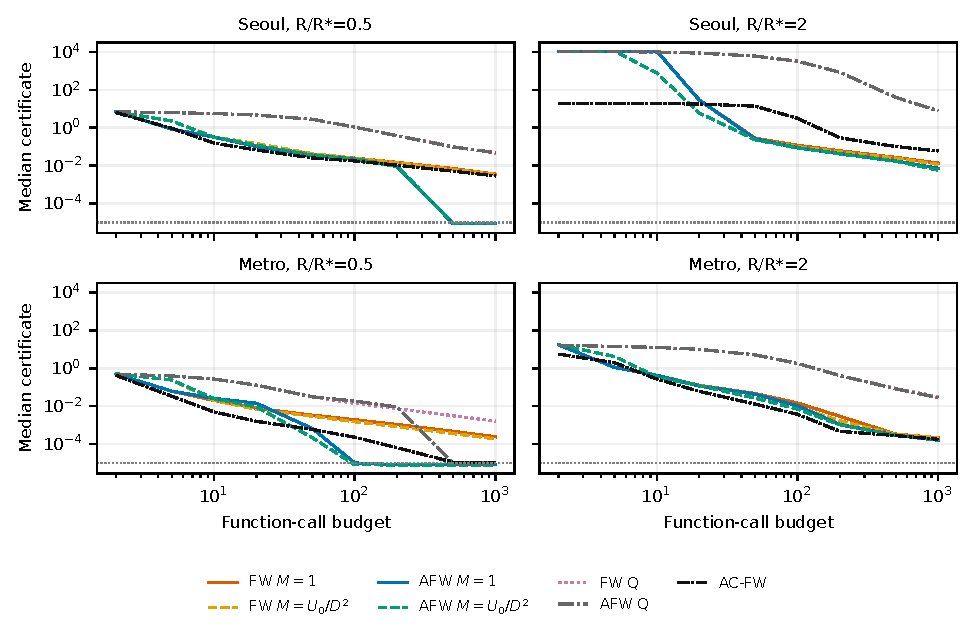
\includegraphics[width=\textwidth]{figures/count_comparators.pdf}
\caption{Median scalar certificates over all distinct vertices at
function-call budgets. Curves include failed runs and charged AC-FW
preprocessing; completed runs are carried forward. The dotted horizontal
line is $10^{-5}$. BT has no curvature inputs, Q receives analytic
$H_0,H_1$. These are paired finite cases, not confidence bands for a
population of problems.}
\label{fig:counts}
\end{figure}

At the active radii, both AFW-BT initializations certify every start at
1000 function calls. FW-BT certifies none on Seoul and only 2/24 or
3/24 on Metro. AC-FW obtains 13/24 active Metro successes and none
on active Seoul. The known-curvature AFW-Q succeeds on all active
Metro starts but none on active Seoul, illustrating conservatism of
the analytic curvature parameters. At the interior radii no method in
this seven-method scalar-certificate comparison reaches the target
within 1000 function calls. End-of-cap results and censored call
medians are reported separately in Table~\ref{tab:counts}.

The references separate remaining error from stopping lag. At the
interior Metro radius, all 24 starts of each BT variant have numerical
reference error upper bound at most $10^{-5}$ by the original endpoint,
but FW has no scalar-certificate successes and AFW has only 6/24 or
7/24. On interior Seoul, the corresponding reference-error condition
holds for 12/30 and 18/30 AFW starts, while neither scalar BT variant
stops. An unsuccessful certificate is therefore not equivalent to a
large remaining primal error.

\subsection{Controlling initialization and objective units}
A separate $2\times2$ study controls the original point versus the
compulsory LMO vertex, and AC versus BT updates. All four cells pay
the same two-source preprocessing, retain both tangent bounds, and
start their first trial at the same secant curvature. Only AC/vertex
is the native published comparator; the other cells isolate factors.
The study contains 280 runs on 70 earlier matched cases and introduces
no new datasets. Table~\ref{tab:init} shows all three planted active
families, including the unfavorable scaled family. Their construction
and the active-face slack identity appear in Appendix~\ref{app:protocol}.

\begin{table}[htbp]
\centering\small
\caption{Starting-point control on three planted active families, ten matched instances each. Counts are certified starts at 1000 function calls. O/V: original point/compulsory initial LMO vertex. The last column is the descriptive paired median BT-V/AC-V certificate ratio and 95\% percentile-bootstrap interval, not a speedup estimate.}
\label{tab:init}
\begin{tabular}{lrrrrl}
\toprule
Family & AC-O & AC-V & BT-O & BT-V & Ratio [interval] \\
\midrule
active & 1 & 10 & 0 & 10 & 1.049 [0.935, 1.257] \\
active\_scaled & 0 & 0 & 0 & 0 & 1.530 [0.822, 1.750] \\
active\_highdim & 6 & 8 & 2 & 8 & 1.231 [0.798, 2.117] \\
\bottomrule
\end{tabular}
\end{table}

On the active family, changing the starting point raises successes
from 1 to 10 for AC and from 0 to 10 for BT. The descriptive
BT/AC certificate-ratio interval from the vertex includes one.
The scaled family remains unsolved by all four controls. Thus the
earlier vertex-start comparison does not isolate an update-rule benefit.

Objective units provide another control. Under $\widetilde f=af+b$,
$a>0$, scaling $M$ and $\varepsilon$ by $a$ preserves the exact
iterates, trials and stopping index, since $G,U,L$ scale together.
Thus $M=U_0/D^2$ is automatically equivariant; fixing its numerical
value instead changes effective initialization. A separate real-data
radius/scale study verifies the counts in all 60 paired scale
comparisons for each certificate-initialized method. This elementary
property does not establish a faster algorithm.

\subsection{Causal stopping controls on fixed BT paths}
We repeat the 432 original BT paths from the count-data study, with
exactly matching original endpoints and oracle counts. Five causal
monitors give 2160 dependent stopping profiles. Disjoint blocks of
$K=8,32,128$ paid affine tangents provide a lower bound using one
additional full LMO per completed block; the scalar envelope is
retained. A separate standard control receives $\mu=0.01$ and uses
$f-\norm{\nabla f}^2/(2\mu)$ as a lower bound. Appendix~\ref{app:monitors}
proves validity and isolated oracle accounting; block sizes are fixed
before outcomes and no monitor reads the reference.

\begin{table}[htbp]
\centering\small
\caption{Isolated causal controls on 432 exactly repeated BT paths, giving 2160 dependent profiles. Counts use each profile's first stop or the original cap. More LMOs compares total direction plus certificate LMOs with scalar. Known $\mu$ receives the analytical ridge coefficient; blocks do not.}
\label{tab:monitors}
\begin{tabular}{lrrr}
\toprule
Profile & Certified & Earlier prefix & More total LMOs \\
\midrule
scalar & 129 & 0 & 0 \\
block\_8 & 129 & 0 & 432 \\
block\_32 & 129 & 0 & 425 \\
block\_128 & 129 & 0 & 380 \\
known\_mu & 226 & 110 & 0 \\
\bottomrule
\end{tabular}
\end{table}

None of the tested blocks gives an earlier stop. The known-$\mu$
control gives 226 successes instead of 129 and 110 earlier prefixes,
with no extra LMOs but additional model information. On interior
Metro each BT variant now reaches 24/24 successes by the original
endpoint; both AFW variants do so within 1000 function calls.
Interior Seoul remains difficult: AFW obtains only 4/30 or 10/30
successes by the endpoint and none at 1000 function calls.
These controls neither establish adaptation to unknown strong convexity
nor evaluate the exact averaged-gradient Fenchel dual in~\cite{pedregosa}.
They show that observable stopping cost is a separate practical issue.


\section{Discussion}
The phase argument replaces a single global curvature bound by a sequence
of source-level bounds while retaining the full feasible-region LMO.
Its output is a guarantee for the accumulated scalar certificate and a
count of every rejected function trial. This distinction matters when a
small primal error is insufficient for an algorithm to certify stopping.
The initialization term is intrinsic to the specified halving rule,
as the affine example shows.

The experiments support controls on initialization, objective units,
and active geometry. They do not establish a universal practical
ranking. Positive $H_1$ on a compact domain does not preclude a global
Lipschitz constant, and the analytic constants can be conservative.
The logarithmic AFW theorem requires its additional geometric
inequality. Exact-arithmetic bounds do not by themselves ensure
finite-precision reliability; deterministic oracle corrections in
Appendix~\ref{app:inexact} only establish certificate validity.
Extending the analysis to controlled noisy directions, pairwise swaps,
and adaptive sliding with all inner linear oracles counted remains open.

\begin{thebibliography}{99}
\bibitem{braun} G.~Braun, A.~Carderera, C.~W.~Combettes, H.~Hassani,
A.~Karbasi, A.~Mokhtari, and S.~Pokutta. Conditional Gradient Methods.
\href{https://arxiv.org/abs/2211.14103v5}{arXiv:2211.14103v5}, 2025.
\bibitem{pedregosa} F.~Pedregosa, G.~Negiar, A.~Askari, and M.~Jaggi.
Linearly Convergent Frank-Wolfe with Backtracking Line-Search.
\emph{AISTATS}, 2020. \href{https://arxiv.org/abs/1806.05123}{arXiv:1806.05123}.
\bibitem{lacostejaggi} S.~Lacoste-Julien and M.~Jaggi.
On the Global Linear Convergence of Frank-Wolfe Optimization Variants.
\emph{NeurIPS}, 2015.
\href{https://arxiv.org/abs/1511.05932}{arXiv:1511.05932}.
\bibitem{warmup} F.~Alimisis, R.~Islamov, and A.~Lucchi.
Why Do We Need Warm-up? A Theoretical Perspective.
\href{https://arxiv.org/abs/2510.03164v2}{arXiv:2510.03164v2}, 2026.
\bibitem{lobanovkoloskova} A.~Lobanov and A.~Koloskova.
Avoiding Bias in Clipped SGD for Overparameterized Models under Generalized Smoothness.
\href{https://arxiv.org/abs/2605.14800v2}{arXiv:2605.14800v2}, 2026.
\bibitem{lobanov} A.~Lobanov.
A Few Accelerated Algorithms for Convex Optimization under $(H_0,H_1)$-Smoothness.
\href{https://arxiv.org/abs/2608.04884}{arXiv:2608.04884}, 2026.
\bibitem{vyguzov} A.~A.~Vyguzov and F.~S.~Stonyakin.
Frank-Wolfe Algorithms for $(L_0,L_1)$-smooth functions.
\href{https://arxiv.org/abs/2510.16468v5}{arXiv:2510.16468v5}, 2026.
\bibitem{selfconcordant} P.~Dvurechensky, K.~Safin, S.~Shtern, and M.~Staudigl.
Generalized Self-Concordant Analysis of Frank-Wolfe Algorithms.
\href{https://arxiv.org/abs/2010.01009}{arXiv:2010.01009}, 2020.
\bibitem{bregmanfw} S.~Takahashi, S.~Pokutta, and A.~Takeda.
Fast Frank--Wolfe Algorithms with Adaptive Bregman Step-Size for Weakly Convex Functions.
\emph{ICLR}, 2026.
\href{https://arxiv.org/abs/2504.04330v4}{arXiv:2504.04330v4}.
\bibitem{adcgs} S.~Takahashi.
Adaptive Conditional Gradient Sliding: Projection-Free and Line-Search-Free Acceleration.
\href{https://arxiv.org/abs/2601.20443v2}{arXiv:2601.20443v2}, 2026.
\bibitem{wirth} E.~Wirth, J.~Pe\~na, and S.~Pokutta.
Fast convergence of Frank-Wolfe algorithms on polytopes.
\href{https://arxiv.org/abs/2406.18789v3}{arXiv:2406.18789v3}, 2025.
\bibitem{restartfw} T.~Kerdreux, A.~d'Aspremont, and S.~Pokutta.
Restarting Frank-Wolfe: Faster Rates under H\"olderian Error Bounds.
\href{https://arxiv.org/abs/1810.02429v4}{arXiv:1810.02429v4}, 2021.
\bibitem{zhao} R.~Zhao.
New Analysis of an Away-Step Frank-Wolfe Method for Minimizing
Logarithmically-Homogeneous Barriers.
\href{https://arxiv.org/html/2305.17808v4}{arXiv:2305.17808v4}, 2023.
\bibitem{autoconditioned} K.-H.~Giang-Tran, S.~Shafiee, and N.~Ho-Nguyen.
Auto-Conditioned Frank-Wolfe Algorithms.
\href{https://arxiv.org/abs/2605.15512}{arXiv:2605.15512}, 2026.
\bibitem{khademi} A.~Khademi and A.~Silveti-Falls.
Adaptive Conditional Gradient Descent.
\href{https://arxiv.org/abs/2510.11440v1}{arXiv:2510.11440v1}, 2025.
\bibitem{yagishita} S.~Yagishita and M.~Ito.
Simple linesearch-free first-order methods for nonconvex optimization.
\href{https://arxiv.org/abs/2509.14670}{arXiv:2509.14670}, 2025.
\bibitem{lacoste2016} S.~Lacoste-Julien.
Convergence Rate of Frank-Wolfe for Non-Convex Objectives.
\href{https://arxiv.org/abs/1607.00345}{arXiv:1607.00345}, 2016.
\bibitem{seoul} Seoul Bike Sharing Demand [Dataset].
UCI Machine Learning Repository, 2020.
\href{https://doi.org/10.24432/C5F62R}{doi:10.24432/C5F62R}. CC BY 4.0.
\bibitem{metro} J.~Hogue. Metro Interstate Traffic Volume [Dataset].
UCI Machine Learning Repository, 2019.
\href{https://doi.org/10.24432/C5X60B}{doi:10.24432/C5X60B}. CC BY 4.0.
\bibitem{karimi} H.~Karimi, J.~Nutini, and M.~Schmidt.
Linear Convergence of Gradient and Proximal-Gradient Methods Under the
Polyak--{\L}ojasiewicz Condition.
\href{https://arxiv.org/abs/1608.04636v4}{arXiv:1608.04636v4}, 2020.
\bibitem{wdbc} W.~Wolberg, O.~Mangasarian, N.~Street, and W.~Street.
Breast Cancer Wisconsin (Diagnostic) [Dataset]. UCI Machine Learning Repository, 1993.
\href{https://doi.org/10.24432/C5DW2B}{doi:10.24432/C5DW2B}.
\bibitem{bike} H.~Fanaee-T. Bike Sharing [Dataset]. UCI Machine Learning Repository, 2013.
\href{https://doi.org/10.24432/C5W894}{doi:10.24432/C5W894}. CC BY 4.0.
\end{thebibliography}

\appendix
\section{Comparison steps and certificate normalization}
\label{app:explicit}
If $H_0,H_1$ are supplied, consider
\[
 \alpha=\min\{1,G/[(H_0+H_1U)q^2]\},
\]
with a full step when its curvature is zero.
Lemma~\ref{lem:local}'s descent argument, with $U\ge\delta$,
gives
\[
 f_k-f_{k+1}\ge\frac12\min\{U_k,U_k^2/[D^2(H_0+H_1U_k)]\}.
\]
In a phase $b/2<U\le b$, progress is at least
$\min\{b/4,b^2/(8D^2H_0+4D^2H_1b)\}$, because the right-hand side
is increasing in $U>0$. The phase budget therefore permits at most
$5+4H_1D^2+8H_0D^2/b$ updates. Summing the same dyadic levels proves
\begin{equation}\label{eq:explicitcount}
 N\le\ceil{(5+4H_1D^2)J+16H_0D^2/\varepsilon}.
\end{equation}
There are $N+1$ calls of each oracle for this explicit step.
Exact segment minimization performs at least as well as the comparison
step, so it inherits~\eqref{eq:explicitcount} without receiving
$H_0,H_1$. This does not bound the inner function or gradient calls
needed for an exact scalar minimizer. The expanded technical report
also derives a hyperbolic step with the same order; its elementary
function is not needed for Theorem~\ref{thm:fw}.

For completeness, certificate-scaled backtracking starts with
$\theta_{-1}=1$, tries $\theta_{k-1}/2$, sets $L=\theta U_k/D^2$,
and doubles $\theta$ on a failed quadratic test. The sufficient
threshold $T_k=D^2(H_0/U_k+H_1)$ is nondecreasing. By induction,
\[
 \theta_k\le\max\{2^{-k-1},2T_k\},\qquad
 L_k\le\max\{U_k/(2^{k+1}D^2),2(H_0+H_1U_k)\}.
\]
Indeed a first-trial acceptance halves the previous bound, and after
a rejection the accepted estimate is less than $2T_k$.
Thus $L_k\le2H_0+(2H_1+1/(2D^2))U_k$. Applying the preceding
phase argument with these effective constants gives
\[
 N\le\ceil{(7+8H_1D^2)J+32H_0D^2/\varepsilon}.
\]
The recursion $\theta_k=2^{r_k-1}\theta_{k-1}$ gives
\[
 N_f\le1+2N+\ceil{\log_2\max\{1,2D^2(H_0/\varepsilon+H_1)\}}.
\]
The last source before an update has $U>\varepsilon$, which bounds
$\theta_{N-1}$. This normalization requires $D$ and is optional for
the two-phase order. Theorems~\ref{thm:fw} and~\ref{thm:afw} concern
ordinary backtracking, rather than this separate variant.

\section{Geometric implications and attaining examples}
\label{app:geometry}
Let $p=\inner{\nabla f(x)}{v-s}$ be the pairwise gap over the full
atom set and current active set. The selected FW/away gap is at
least $p/2$. The standard polytope scaling inequality gives, for
any optimal $x^*\ne x$,
\[
 p\ge W\frac{\inner{\nabla f(x)}{x-x^*}}{\norm{x-x^*}}.
\]
See~\cite[Theorem 3]{lacostejaggi} and
\cite[Lemmas 3.4 and 3.6]{restartfw}. For quadratic growth, choose
a nearest optimum. Convexity and the growth inequality imply
$p\ge W\delta/\operatorname{dist}(x,X^*)
\ge W\sqrt{\gamma\delta/2}$. Hence
$g^2\ge\gamma W^2\delta/8$, giving $\kappa=\gamma W^2/16$.
Monotone iterates stay in the initial sublevel set where growth is
assumed. No uniqueness is required. For strong convexity,
$\inner{\nabla f(x)}{x-x^*}\ge\delta+\mu\norm{x-x^*}^2/2$;
minimizing $\delta/r+\mu r/2$ over $r>0$ gives
$p\ge W\sqrt{2\mu\delta}$ and $\kappa=\mu W^2/4$.
These geometric implications are prior results.

\subsection{Gap-envelope equality and zero base curvature}
\label{app:bridge}
Let $Q=[-D/2,D/2]$, $x=D/2$ and $f(y)=h(y-z)^2/2$, $h>0$.
For $z\in Q$, $\delta=h(x-z)^2/2$ and
$G=hD(x-z)=\sqrt{2hD^2\delta}$, attaining the square-root branch
of~\eqref{eq:sharpbridge} with $H_0=h,H_1=0$.
For $z<-D/2$, the constrained optimum is $-D/2$,
$\delta=-hDz$ and $G=\delta+hD^2/2$, attaining its full-step branch.
This proves sharpness for that quadratic descent inequality, not an
optimal envelope over all functions satisfying~\eqref{eq:curvature}
with $H_1>0$.

The example $f(x)=t+t^3$, $t=1/2-x\in[0,1]$, has
$f''(x)=6t\le6f(x)$, so $H_0=0,H_1=6$.
It is not strongly convex. At a nonoptimal interior point both
endpoint atoms are active, and the selected gap is
$(1+3t^2)\max\{t,1-t\}\ge1/2$; the nonoptimal endpoint also satisfies
this inequality. Since $\delta\le2$, condition~\eqref{eq:geometry}
holds with $\kappa=1/16$. At zero error the geometric inequality is
immediate. This shows the $H_0=0$ extension is nonvacuous.

\section{Lower-bound controls and deterministic oracle errors}
\label{app:monitors}
Write $g_j=\nabla f(x_j)$ and $a_j=f(x_j)-\inner{g_j}{x_j}$.
For a completed block $B$ of $K$ consecutive paid sources,
\[
 b_B=\bar a_B+\min_{v\in Q}\inner{\bar g_B}v\le f_Q^*.
\]
Convexity gives $f(v)\ge a_j+\inner{g_j}v$ for each source;
average and minimize to prove validity. Disjoint blocks begin at
source zero, and an incomplete block is not queried. The new lower
bound is the maximum of $\ell_k$ and all completed $b_B$.
Its certificate is nonincreasing and at most $U_k$ on the same
monotone path, so its first crossing occurs no later in updates,
function or gradient calls. At source $k$, exactly
$\lfloor(k+1)/K\rfloor$ additional full LMOs have been performed.
Total LMO cost need not decrease. The monitors affect neither the
line search nor the initial $M$; each reported cost is for one
isolated monitor, excluding the other diagnostic monitors.
An affordable budget source pays its entire scheduled verification.

These uniform block bounds differ from the averaged-gradient Fenchel
dual in~\cite[Theorem 3]{pedregosa}. When the global conjugate exists,
Fenchel equality and Jensen give
\[
 b_B=-\overline{f^*(g_j)}-\sigma_Q(-\bar g_B)
     \le-f^*(\bar g_B)-\sigma_Q(-\bar g_B).
\]
Here $f^*$ denotes the conjugate, not the scalar optimum $f_Q^*$.
No transfer of that paper's theorem or averaging weights is asserted.
With a valid supplied strong-convexity constant $\mu$,
$f(x_j)-\norm{g_j}^2/(2\mu)\le f_Q^*$ follows by minimizing the
quadratic lower model over $\R^d$~\cite[Appendix B]{karimi}.
Caching these bounds costs no LMO, but uses additional information.
Native stopping checks on one synthetic interior instance verify all
20 method/profile pairs against the attainable-prefix construction
and instrument actual oracle calls. They do not represent 2160
additional native solver runs.

\subsection{Certificate validity with bounded deterministic errors}
\label{app:inexact}
If $|\widehat f-f(x)|\le\nu$,
$\norm{\widehat g-\nabla f(x)}\le\rho$ and
$\inner{\widehat g}s\le\min_{v\in Q}\inner{\widehat g}v+\eta$
with known bounds, then
\[
 \ell^{\rm safe}=\widehat f+\inner{\widehat g}{s-x}
                      -\nu-\rho D-\eta\le f_Q^*.
\]
For each $v\in Q$, convexity gives
$f(v)\ge\widehat f-\nu+\inner{\widehat g}{v-x}-\rho D
\ge\ell^{\rm safe}$; minimize over $v$.
A maximum of such lower bounds remains valid, and
$\widehat f+\nu-\max_j\ell_j^{\rm safe}$ is an upper certificate.
This is a validity statement, not a convergence theorem for noisy
directions. Empirical variance is not a deterministic norm bound.

\section{Additional protocol details and controls}
\label{app:protocol}
\paragraph{Features.}
Seoul uses eight numerical weather features (temperature, humidity,
wind speed, visibility, dew point, solar radiation, rainfall and snowfall),
sine/cosine of hour and weekday, holiday and functioning indicators.
Metro uses temperature, rain, snow, cloud cover, sine/cosine of hour,
weekday and day of year (period 365.25), and a holiday indicator.
Other textual categories are omitted. Features constant on training
data are dropped before the $\tanh$ transform; source encodings and
feature names are recorded in the manifests. These deterministic
choices precede the solver comparisons.

\paragraph{Native comparator.}
For $x\ne y$, the AC-FW estimate is
\[
 \ell(x,y)=\frac{2|f(y)-f(x)-\inner{\nabla f(x)}{y-x}|}{\norm{y-x}^2},
\]
and it is zero if $x=y$. Its update is the maximum of this trial estimate
and $r_kL_k$, with $r_k=1-1/((k+1)\log^2(k+3))$.
Only strict objective decrease accepts a trial.
After $N$ outer trials the charged counts are
$N_f=N_{\rm LMO}=N+2$, $N_g=N_{\rm accepted}+2$.
Rejected trials count against the cap. All primary count-data starts
are atoms, as in the cited initialization. Parameter-hidden tests on
both count datasets instrument preprocessing, rejected trials and
oracle calls independently of recorded counters.

\paragraph{Planted geometry.}
For the initialization controls, let
\[
 \phi(x)=m^{-1}\sum_i[\cosh(a_i^\top(x-x^*))-1]
                         +\mu\norm{x-x^*}^2/2,
 \quad f(x)=\phi(x)-\lambda v^\top(x-x^*),
\]
where $\norm{x^*}_1=R$, $v\in\partial\norm{x^*}_1$ and
$\lambda=0.15$. On $Q$, $f\ge\phi\ge0=f_Q^*$ and
$\nabla f(x^*)=-\lambda v\ne0$. Valid constants are
$H_0=\mu+\lambda_{\max}(A^\top A/m)$ and
$H_1=\max_i\norm{a_i}^2$.
The active and active-scaled families use $d=12,m=10$,
$R=1.5,\mu=0.08$, with $x^*$ entries $(0.6,-0.5,0.4)$ at
coordinates $(2,6,10)$; Gaussian row entries have standard deviation
$0.22$ or $0.9$. The high-dimensional family has $d=60,m=40$
and standard deviation $0.22$. Each has ten matched seeds.
Off-support normal coordinates are uniform in $[-0.6,0.6]$.

With $w=\operatorname{sign}(x^*)$, zero off support, the optimal-face
slack $\sigma(x)=R-w^\top x$ obeys
$\sigma(x+\alpha(s-x))=(1-\alpha)\sigma(x)+\alpha\sigma(s)$.
Thus strict subunit steps to atoms on the face keep positive slack
from an exterior start. A full initial vertex move can remove it.
Moreover $f(x)\ge0.4\lambda\sigma(x)$ on these planted examples.
This familiar FW face obstruction explains why initialization is a
necessary control, not a new acceleration mechanism.

\paragraph{Objective-unit study.}
The separate radius/scale archive contains 360 runs on the WDBC
logistic control and UCI Bike Sharing Poisson objective~\cite{wdbc,bike},
three radii, five seeds, three positive scales
and four BT methods. Accuracy is scaled with the objective.
The 60 pairwise scale comparisons per certificate-initialized method
compare final counters and sampled budget certificates, not bitwise
identity of every intermediate iterate. All scalings of a problem
are dependent controls. Additional studies and full baseline settings
are retained in the expanded technical report and companion archive.

\begin{table}[htbp]
\centering\small
\caption{Certification at $10^{-5}$ within 1000 updates. Each cell gives the certified count and median function calls to stop or cap, including failed runs. Seoul has 30 starts and Metro 24 per radius/method. $F/A$: FW/AFW; subscripts $1,U$: BT initialized at $1,U_0/D^2$; $Q$: known-$H$ short step. AC counts 1000 outer trials, including rejections, and pays two preprocessing source evaluations. These medians are not times to success.}
\label{tab:counts}
\begin{tabular}{llrrrrrrr}
\toprule
Data & $R/R_*$ & $F_1$ & $F_U$ & $A_1$ & $A_U$ & $F_Q$ & $A_Q$ & AC \\
\midrule
Seoul & 0.5 & 1; 2001 & 1; 2003 & 30; 424 & 30; 399 & 0; 1001 & 0; 1001 & 0; 1002 \\
Seoul & 2 & 0; 2001 & 0; 1996 & 0; 2001 & 0; 1995.5 & 0; 1001 & 0; 1001 & 0; 1002 \\
Metro & 0.5 & 3; 2001 & 3; 2003 & 24; 99 & 24; 80.5 & 1; 1001 & 24; 423 & 13; 385 \\
Metro & 2 & 0; 2000 & 0; 2002 & 6; 2000 & 7; 2001 & 0; 1001 & 0; 1001 & 0; 1002 \\
\bottomrule
\end{tabular}
\end{table}


\section{What the closest bounds directly establish}
\label{app:comparison}
The following comparison concerns specific stated results, not every
possible consequence of their proofs.
Khademi and Silveti-Falls~\cite[Theorems 4.4--4.5]{khademi}
combine gradient-difference estimates with backtracking. Their stated
constrained rates retain a global smoothness/gradient contribution;
they also explicitly discuss slow downward adaptation of ordinary
backtracking. Thus that motivation is prior. Yagishita and
Ito~\cite[Algorithm 3, Theorem 3.1]{yagishita} analyze a line-search-free
composite conditional-gradient method with a nondecreasing estimate
and a nonconvex minimum-gap guarantee. These are different methods
and stopping statements, not evidence for a general priority claim.
Pedregosa et al.~\cite[Theorem 3]{pedregosa} bound a last-iterate
Fenchel primal--dual gap using averaged accepted curvature estimates.
Its dual lower value and the maximum scalar tangent lower bound have
no general ordering for arbitrary histories: for $f=x^2/2$ on
$[-1,1]$, histories $(-1,1)$ and $(-1,-1/2)$ reverse the order.
These histories are not asserted to be algorithm trajectories and do
not contradict that theorem. Its Theorem 4 already yields geometric
progress from accepted local curvature, which our AFW proof specializes.

Substituting $L_Q=H_0+H_1\max_Q\delta$ in a global smoothness bound
retains the global gap range. The smaller initial certificate $U_0$
does not bound curvature everywhere on $Q$; restricting the region
to an initial sublevel set would change its LMO.
Our first-return argument instead bounds only the tested descent
segment. A phase count controls estimates above the current level.

The deterministic convex result in~\cite[Appendix C.4]{lobanovkoloskova}
already separates function-dependent-curvature regimes for gradient
descent; it is not an LMO certificate theorem.
The gradient-norm dependent FW analysis in~\cite[Theorem 5.1]{vyguzov}
contains a largest-gradient contribution after a direct substitution.
Neither the use of phases nor unknown-curvature adaptation alone
is presented as new here.

Takahashi et al.~\cite{bregmanfw} use relative smoothness, a kernel,
and segment scaling. A Euclidean kernel with a single global $L_Q$
does not by itself give the separated dependence above.
For adaptive sliding~\cite[Theorems 2.1 and 4.1]{adcgs}, inner LMO
effort is distinct from outer iterations, and the restarted theorem
also requires local strong convexity and its scheduling parameters.
Condition~\eqref{eq:curvature} alone does not give strong convexity:
$\cosh(x_1)-1$ on a square has a line of minimizers.
No superiority over sliding is established.

Wirth et al.~\cite[Definition 2.3(b), Theorem 3.6]{wirth} use uniform
extended curvature and a vertex error bound. Kerdreux et
al.~\cite[Proposition 4.2, Theorem 5.1]{restartfw} already combine
burn-in, computable strong-Wolfe stopping, unknown error-bound
parameters and cumulative LMO counts, with global away curvature.
Zhao~\cite[Theorems 4.1--4.2]{zhao} proves linear objective- and
FW-gap rates for log-homogeneous barriers, using exact search or a
local-Hessian step. Our function class and the evaluated algorithm
differ. None of these comparisons rules out an equivalent refined
specialization of another adaptive proof.

\section{Reproducibility and evidence checks}
\label{app:reproduction}
The companion package includes source snapshots, raw data attribution,
CSV results and SHA-256 manifests. The main real-data comparison
joins 648 preserved records with 108 additional AC-FW records on the
same cases; it does not count them as new datasets.
The certificate study replays 432 existing paths and reports 2160
dependent causal profiles. The initialization factorial also reuses
earlier cases. Table values are generated from immutable CSVs; the
claim ledger records each selection and its value.

The recorded environment uses Python 3.13.5, NumPy 2.5.2, SciPy 1.16.3,
Matplotlib 3.10.9 and scikit-learn 1.8.0, with BLAS/OpenMP thread
environment variables set to one. From the extracted repository root:
\begin{verbatim}
python -m pip install -r PART3/requirements.txt
python -m unittest discover -s PART3/Work -p "test_*.py"
python PART3/Work/validate_results.py
python PART3/Paper/prepare_article_evidence.py
\end{verbatim}
The 58 tests cover derivatives, reference independence, actual oracle
calls, certificates, accepted progress and curvature limits. Full
trajectory audits run before trace sampling; saved validators also
check provenance and budget accounting.
A separate finite audit uses exact rational arithmetic for 8370
phase configurations, 57989 abstract curvature-state visits, phase
budgets, gap inversion and atom-removal counts. It overapproximates
possible curvature histories and does not assert that every state
is realizable by an objective. Finite tests are not a formal proof
or independent mathematical review.

The broader legacy experiments include repeated Bike Sharing initial
vertices: ten historical seeds give seven distinct starts. Later
activity-sweep summaries explicitly remove those duplicates. Those
historical seed-weighted summaries are not used as independent
replications in the main count-data comparison, which enumerates all
distinct vertices. Numerical references and floating-point audits
do not provide directed-rounding guarantees.

\paragraph{Generative-tool disclosure.}
An OpenAI Codex assistant was used substantially for literature triage,
proof development, implementation, experiment analysis, manuscript
drafting and verification automation. The explicit derivations, source
snapshots and executable checks are supplied for scrutiny. Automated
checks and AI-assisted internal review are not independent mathematical
peer review. Responsibility for the submitted scientific claims rests
with the named authors.

\end{document}
